\documentclass{report}
\usepackage[utf8]{inputenc}
\usepackage{color}   %May be necessary if you want to color links
\usepackage{hyperref}
\usepackage{graphicx}
\usepackage{subcaption}
\graphicspath{ {./graphs/} }
\hypersetup{
	linkcolor=blue,
	citecolor=blue,
	urlcolor=blue,
}
\title{\textbf{Patterns of Crime and Arrest Disparities in Tucson: A Multivariate Perspective}}
\author{Nathan Tebbs \and Andrew Hicks \and Cole Hageman}
\date{\today}



\begin{document}
\maketitle
\tableofcontents


	\chapter{Introduction}
	
	In this project, we are studying how environmental and socioeconomic factors affect crime and arrest patterns in neighborhoods across Tucson, Arizona. Crime is not evenly spread throughout a city, and some areas may experience more police activity or higher arrest rates than others. We want to understand if these differences are related to things like income, housing values, or access to infrastructure such as street lighting.
	
	Our main goal is to find out whether certain neighborhood conditions are linked to higher crime or arrest rates. We also want to see if there are patterns in the data that suggest some areas are policed more heavily than others, even when crime levels are similar. These questions are important for making sure public safety policies are fair and based on evidence, not just assumptions.
	
	\newpage
	\section{Objectives}
	
	To study this, we are using public datasets from the City of Tucson. These include records of reported crimes and arrests, information about neighborhood income levels and housing values, and data about streetlights and other infrastructure. By combining these sources, we hope to conduct a comparative analysis between these different. Our research questions are as follows:
	
	\begin{itemize}
		\item Do thefts and violent crimes occur more often in richer or poorer neighborhoods?
		\item Does the existance or prescence of city streetlights influence crime rates
	\end{itemize}
	
	\section{Overview of Data}
	
	This project uses multiple datasets to explore how socioeconomic and environmental conditions are related to crime and arrest disparities in Tucson neighborhoods. Each dataset supports a specific part of our analysis, allowing us to examine relationships between location-based factors, community demographics, and law enforcement activity.
	
	\begin{enumerate}
		\item \textbf{Tucson Police Reported Crimes}
		\par This dataset provides detailed records of reported crimes within the City of Tucson. Each entry includes the type of crime, the location, and the date and time of the report. This data will be used to analyze spatial and temporal patterns of criminal activity at the neighborhood level.
		
		\item \textbf{Tucson Police Arrests}
		\par The arrests dataset contains information on individual arrests made by Tucson Police, including the offense type, arrest location, and demographic details of the individuals arrested. This dataset is central to our analysis of disparities in arrest rates across neighborhoods with different socioeconomic profiles.
		\item \textbf{City of Tucson Streetlight Locations}
		\par This dataset contains the locations of public streetlights across Tucson. We will use it to examine whether infrastructure quality—particularly nighttime visibility—correlates with crime or arrest patterns. It will also support our environmental analysis by identifying areas with limited lighting.
		
		\item \textbf{Neighborhood Income}
		\par Neighborhood-level income data is drawn from a publicly available CSV that aggregates income estimates, likely based on census tract boundaries. This data will help us evaluate the economic conditions of each area and investigate how they relate to both crime rates and arrest disparities.
		
		
	\end{enumerate}
	
	
	
	\section{Related Works}
	
	The foundation of our project is supported by past research that explores the complex relationship between neighborhood-level conditions and disparities in crime and arrest patterns. Two key studies inform our approach to understanding how environmental and socioeconomic factors shape community-level justice outcomes.
	\subsection{“The Effects of Neighborhood Characteristics on Police Officers’ Decisions to Initiate Encounters” by Robin S. Engel, Michael R. Smith, and Robert E. Worden (2007)}
	Published in Criminology, this study examines how the socioeconomic and demographic composition of neighborhoods influences police decision-making. Using observational data of police-citizen interactions, Engel et al. analyze whether officers are more likely to initiate contact in certain types of neighborhoods. Their findings indicate that areas with higher levels of disadvantage and minority population are more heavily policed, independent of actual crime levels. This research is important to our project because it shows that neighborhood characteristics, such as poverty, racial composition, and disorder, may contribute to disparities in police behavior and arrest rates regardless of actual crime. It supports the idea that structural factors can shape law enforcement patterns across different parts of a city, which connects directly to our goal of examining arrest disparities in Tucson neighborhoods.
	
	\subsection{“Predictive Policing: The Argument for Public Transparency” by Sarah Brayne (2008)}
	This report from the Campbell Collaboration reviews the rise of predictive policing technologies and how they are often implemented without transparency. The study highlights that these tools typically rely on historical crime and arrest data, which may reflect existing biases. As a result, predictive systems can reinforce patterns of over-policing in low-income or minority communities. Brayne argues for increased accountability and public access to the data and algorithms that drive these systems. This research helps guide the ethical framework of our project. While we aim to uncover statistical relationships between neighborhood conditions and arrest rates, we are also aware of the limitations and risks that can come with interpreting such data without proper context.
	
	\newpage
	\section{Methods and Techniques}
	
	lorem ipsum
	
	\section{Evaluation Framework}
	
	lorem ipsum
	
	\section{Software and Tools}
	
	lorem ipsum \ref{fig:crime-type-by-ward}
	
	\chapter{Exploratory Data Analysis}

        \begin{figure}[!t]
          \begin{subfigure}{1.0\textwidth}
            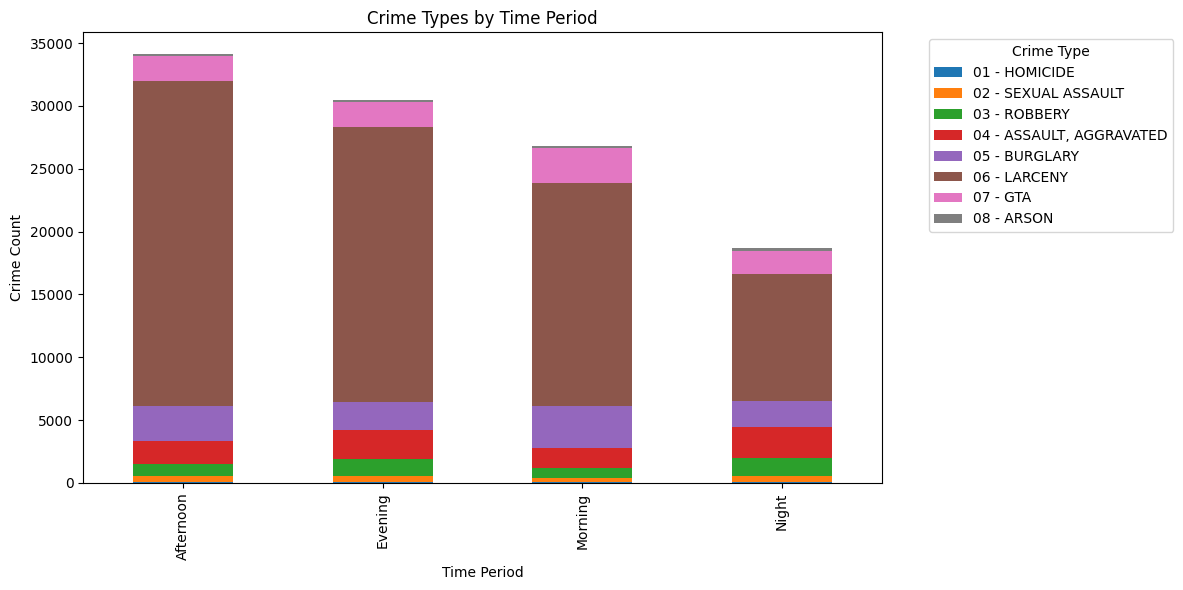
\includegraphics[width=1.25\linewidth, height=8cm, scale=1.5]{crime-types-by-time}
            \caption{Prevalence of Crime Types Across Different Time Periods}
            \label{fig:crime-type-by-time}
          \end{subfigure}
          \begin{subfigure}{1.0\textwidth}
            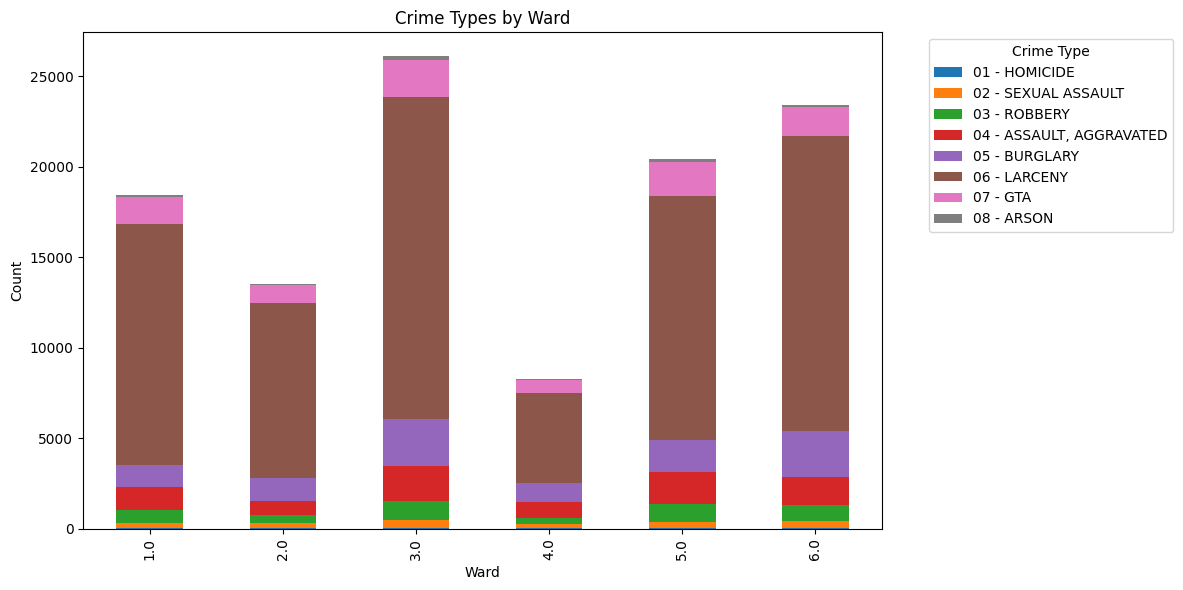
\includegraphics[width=1.25\linewidth, height=8cm]{crime-types-by-ward}
            \caption{Dominant Crime Types by Ward}
            \label{fig:crime-type-by-ward}
          \end{subfigure}
          \caption{Comparing Crime Statistics by Time and Ward}
        \end{figure}
	
	
\end{document}
